Como en el punto 1 del tp se generan casos de pruebas aleatoreos

Este genera instancias con 100 edificios con comienzos, alturas y finalizaciones aleatorias.

\begin{figure}[H]
\begin{center}
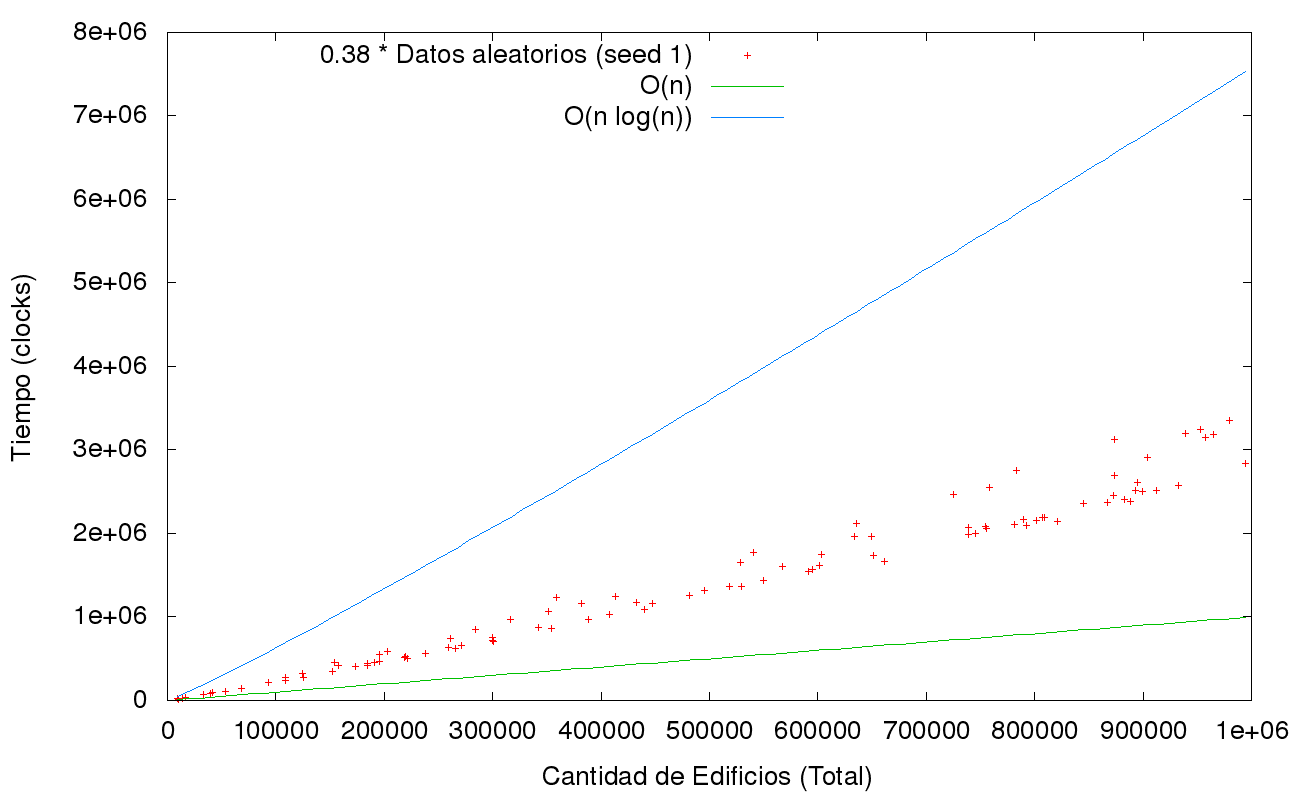
\includegraphics[scale=0.35]{./imagenes/ej2_chartRendimiento.png}
\caption{Gr\'afico de tiempo en funci\'on de la cantidad de edificios.}
\end{center}
\end{figure}

Para evidenciar que la complejidad es la que propusimos en el análisis teórico en el gráfico agregamos dos funciones para acotar superior e inferiormente. Una O(nlog(n)) y la otra O(n).